\documentclass[a4paper]{article}

\usepackage[spanish]{babel}
\usepackage[utf8]{inputenc}
\usepackage{xcolor}
\usepackage[hyphens]{url}
\usepackage[colorlinks=true, urlcolor=black]{hyperref}
\usepackage{graphicx}

\definecolor{shadecolor}{RGB}{220,220,220}

\title{Informe CSV jMeter test}

\date{}

\begin{document}
\setlength{\voffset}{-1in}
\setlength{\textheight}{680px}
\setlength{\headsep}{30px}
\pagenumbering{gobble}
\maketitle

\section{Objetivo}

Como explica el enunciado de este A+, jMeter usa siempre los mismos datos para todos los hilos, que son los datos que se guardan al grabar la traza del caso de uso. Esto puede ser un inconveniente para algunos caso de uso. Por poner un ejemplo, si queremos comprobar el rendimiento de un caso de uso de borrado y se utilizan los mismos datos para todos los hilos, todos entraran bajo el mismo usuario, el primero borrara el elemento, y el resto intentará realizar un borrado de un objeto que ya no existe en base de datos.

\section{Configuración}

La configuración de jmeter es muy simple. Por un lado, necesitmamos un archivo CSV, en el que vamos a poner varias filas de datos. Cada hilo tomará los datos de una fila diferente. Además, en cada fila se deben recoger todos los parámetros necesarios para el caso de prueba en cuestión. Si queremos por ejemplo que, como en el ejemplo anterior, cada hilo entre con un usuario diferente y borre un mensaje de su cuenta, necesitariamos poner usuario, contraseña y id del mensaje a borrar separados por coma en cada fila. Al tener en nuestro caso mismo usuario y contraseña nos bastaría con dos parametros en total por fila. 

\begin{figure}[h!]
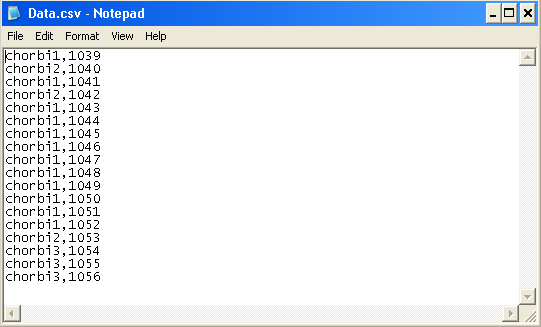
\includegraphics[width=\linewidth]{Data}.
  \caption{Archivo CSV.}

\end{figure}

Después necesitaríamos configurar jMeter para que lea este fichero. Para ello agregamos en nuestro \textit{test plan} el elemento de configuración \textit{CSV Data set config}.

\begin{figure}[h!]
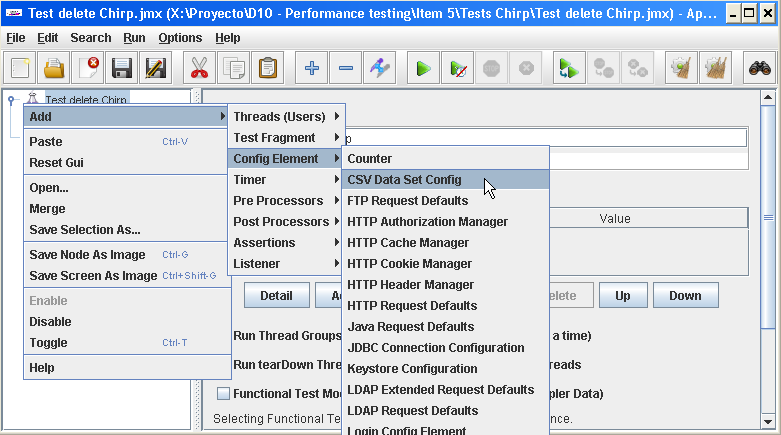
\includegraphics[width=\linewidth]{menu_csv}.
  \caption{Menu para añadir el elemento.}
\end{figure}

Tenemos que configurar en el elemento añadido cuales van a ser las variables a las que se les asignen los distintos valores del csv y cuales en que ruta esta dicho csv. Hay otra opciones que se explican con más detalle en la documentación que se proporciona en el primer link de la bibliografía. Por ejemplo. \textit{Recycle on EOF} puesto a \textit{true} provocará que una vez terminado el fichero, se vuelva al principio de este, mientras que a \textit{false} el comportamiento dependera del valor de \textit{Stop thread on EOF}, asignando un valor por defecto o parando al hilo al llegar al final del documento.

\begin{figure}[h!]
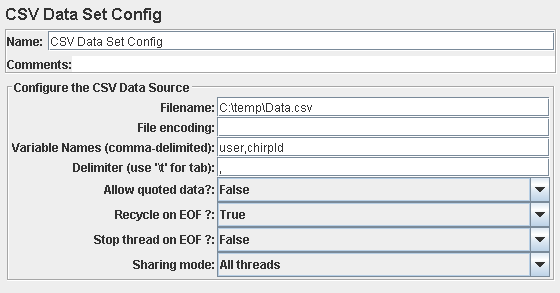
\includegraphics[width=\linewidth]{Config1}.
  \caption{Configuración del elemento.}
\end{figure}

Ahora debemos grabar un caso de uso con normalidad, y una vez que lo tengamos, tenemos que editar el login y el borrado para añadir nuestros parámetros en vez de lo que se ha grabado. En nuestro caso tenemos que modificar el \textit{/j\_spring\_security\_check}, el \textit{/chirp/chorbi/view.do} y el \textit{/chirp/chorbi/delete.do}. En cada caso, tenemos que modificar los \textit{values} por los parametros, con el formato \$\{nombre\_del\_parámetro\}

\begin{figure}[h!]
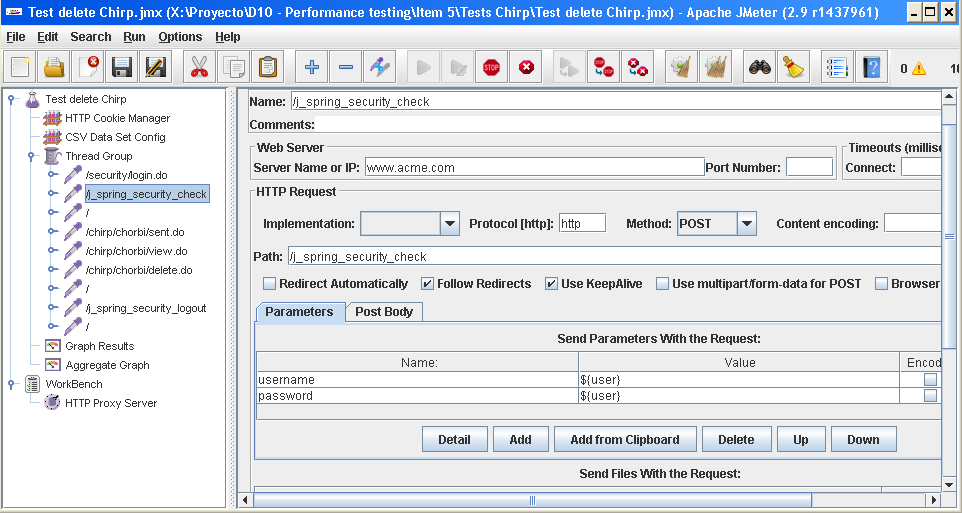
\includegraphics[width=\linewidth]{Config2}.
  \caption{j\_spring\_security\_check}
\end{figure}

\begin{figure}[h!]
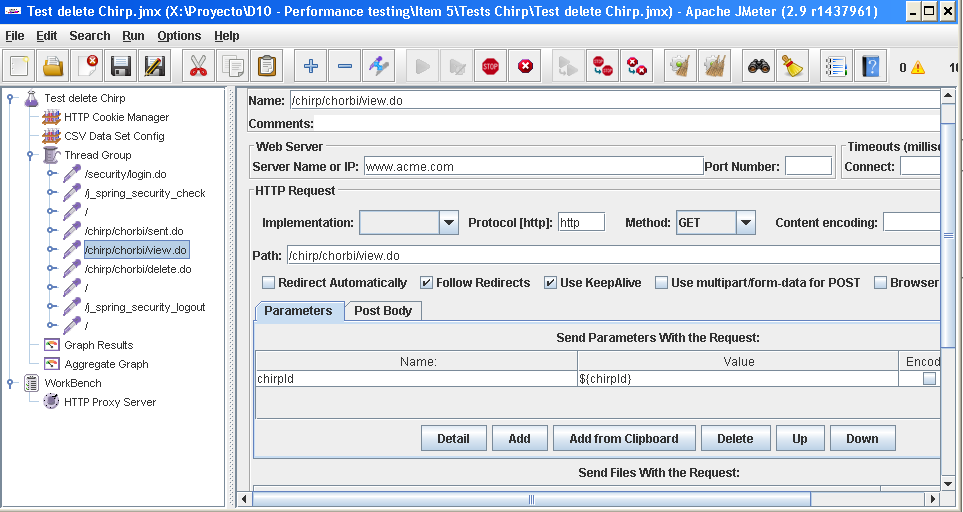
\includegraphics[width=\linewidth]{Config3}.
  \caption{chirp/chorbi/view.do}
\end{figure}

\begin{figure}[h!]
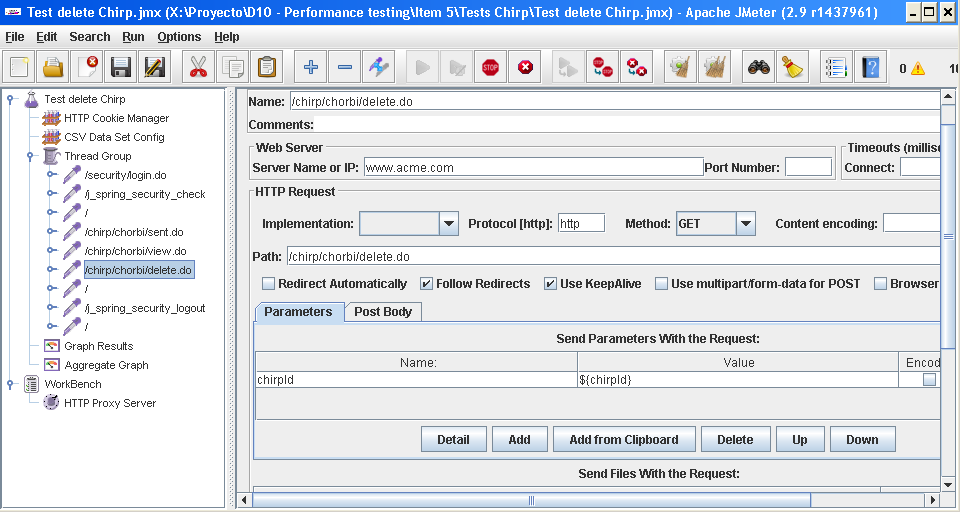
\includegraphics[width=\linewidth]{Config4}.
  \caption{chirp/chorbi/delete.do}
\end{figure}

\section{Problemas y posibles mejoras}

Tal y como esta planteado, la interacción del test depende por completo de los datos que ya existen. No podemos, por ejemplo, crear un nuevo objeto y eliminarlo, ya que la eliminación dependerá del ID del objeto creado, y no podemos saber de antemano que ID se eligirá al crear el objeto. Como nos pasaba, la primera vez se borrará, y el resto intentará borrar un objeto que ya no existe (o incluso que no pertenece al usuario que lo esta intentando, si hemos parametrizado varios usuarios). Para conseguir que los test sean dinámicos necesitariamos guardar en una variable la ID del objeto nuevo y usar esa variable para el borrado. Conseguir capturar esta ID y utilizarla como parámetro puede ser un A+ aun más interesante que el abordado.

\section{Bibliografía}
\url{http://jmeter.apache.org/usermanual/component_reference.html#CSV_Data_Set_Config}

\url{http://ivetetecedor.com/how-to-use-a-csv-file-with-jmeter/}
\end{document}